\documentclass[convert, tikz, border=5pt]{standalone}
\usetikzlibrary{positioning, calc}

\begin{document}

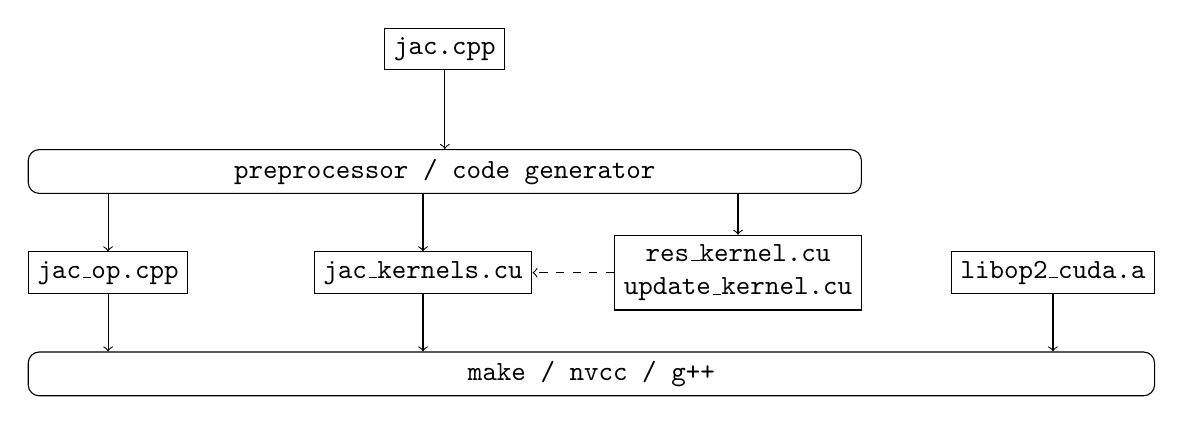
\begin{tikzpicture}[every node/.style={draw, font=\tt}, node distance=4cm, align=center]
    \node (jacop)      []                    {jac\_op.cpp};
    \node (jackernels) [right of=jacop]      {jac\_kernels.cu};
    \node (kernels)    [right of=jackernels] {res\_kernel.cu\\update\_kernel.cu};
    \node (libraries)  [right of=kernels]    {libop2\_cuda.a};

    \path let
        \p1=(jacop.west),
        \p2=(kernels.east)
    in node (preprocessor) [
        rounded corners,
        above=1cm of jacop.west, anchor=south west, minimum width=\x2-\x1-\pgflinewidth
    ] {preprocessor / code generator};

    \node (jac) [above=1cm of preprocessor] {jac.cpp};

    \path let
        \p1=(jacop.west),
        \p2=(libraries.east)
    in node (build) [
        rounded corners,
        below=1cm of jacop.west, anchor=north west, minimum width=\x2-\x1-\pgflinewidth
    ] {make / nvcc / g++};

    \draw[->] (jac)        -- (preprocessor);

    \draw[<-] (jacop)      -- (jacop      |- preprocessor.south);
    \draw[<-] (jackernels) -- (jackernels |- preprocessor.south);
    \draw[<-] (kernels)    -- (kernels    |- preprocessor.south);

    \draw[->] (jacop)      -- (jacop      |- build.north);
    \draw[->] (jackernels) -- (jackernels |- build.north);
    \draw[->] (libraries)  -- (libraries  |- build.north);

    \draw [dashed, ->] (kernels) -- (jackernels);
\end{tikzpicture}

\end{document}
